
\chapter{INTRODUCTION}

Co-channel speech refers to single-channel audio signals that contain more than one speaker. 
The presence of speech interference is an important artifact for all automatic speech processing systems. 
As speech technology advances into our daily lives (in the form of text-to-speech recognition, speaker verification systems), the need to address multi-speaker interference increases. 
Unfortunately, despite its long history, little advancement has been achieved in dealing with co-channel speech. 
This is partly due to the non-stationary nature of speech interference. 
Speech is a dynamic signal with both short-term and long-term changes in a person's voice. 
Adding more speakers to the problem, only increases the difficulty of addressing speech processing. Hence for a long time, co-channel speech has been left under the radar. 
The current state of speech technology has turned co-channel speech into everyone's problem. 
Speech recognition is enabled in most smart-phones. 
During the course of this study, the two most popular operating systems had been released with in-built speech recognizers and one comes with a voice-based user verification system. 
These are signs that current speech technology is extending its reach into our daily activities. 
The existence of this study is due in part to the rise of a new age in speech technology where speech research is not limited to isolated single-speaker conditions. 


A wide range of terms have been used to describe various aspects of co-channel speech, 
which will be clarified throughout this chapter. 
This study addresses both conversational speech and artificially mixed audio streams as co-channel. 
Although some studies propose multi-channel solutions to co-channel speech~\cite{panahi2009blind,xiao2011overlapped}, the focus here is solely on single-channel recordings (i.e., a single microphone). 
In co-channel data, a subset of instances may contain more than one ``active'' speaker at the same time, i.e. multi-speaker segments, 
which we label as ``overlapped speech''. 
Overlapped regions are segments of a co-channel signal where both speakers are simultaneously active. This categorization is summarized in Fig.~\ref{fig:cochannel_vs_overlap}.


\begin{figure}[h!]
	\centering
	\vspace{0mm}
	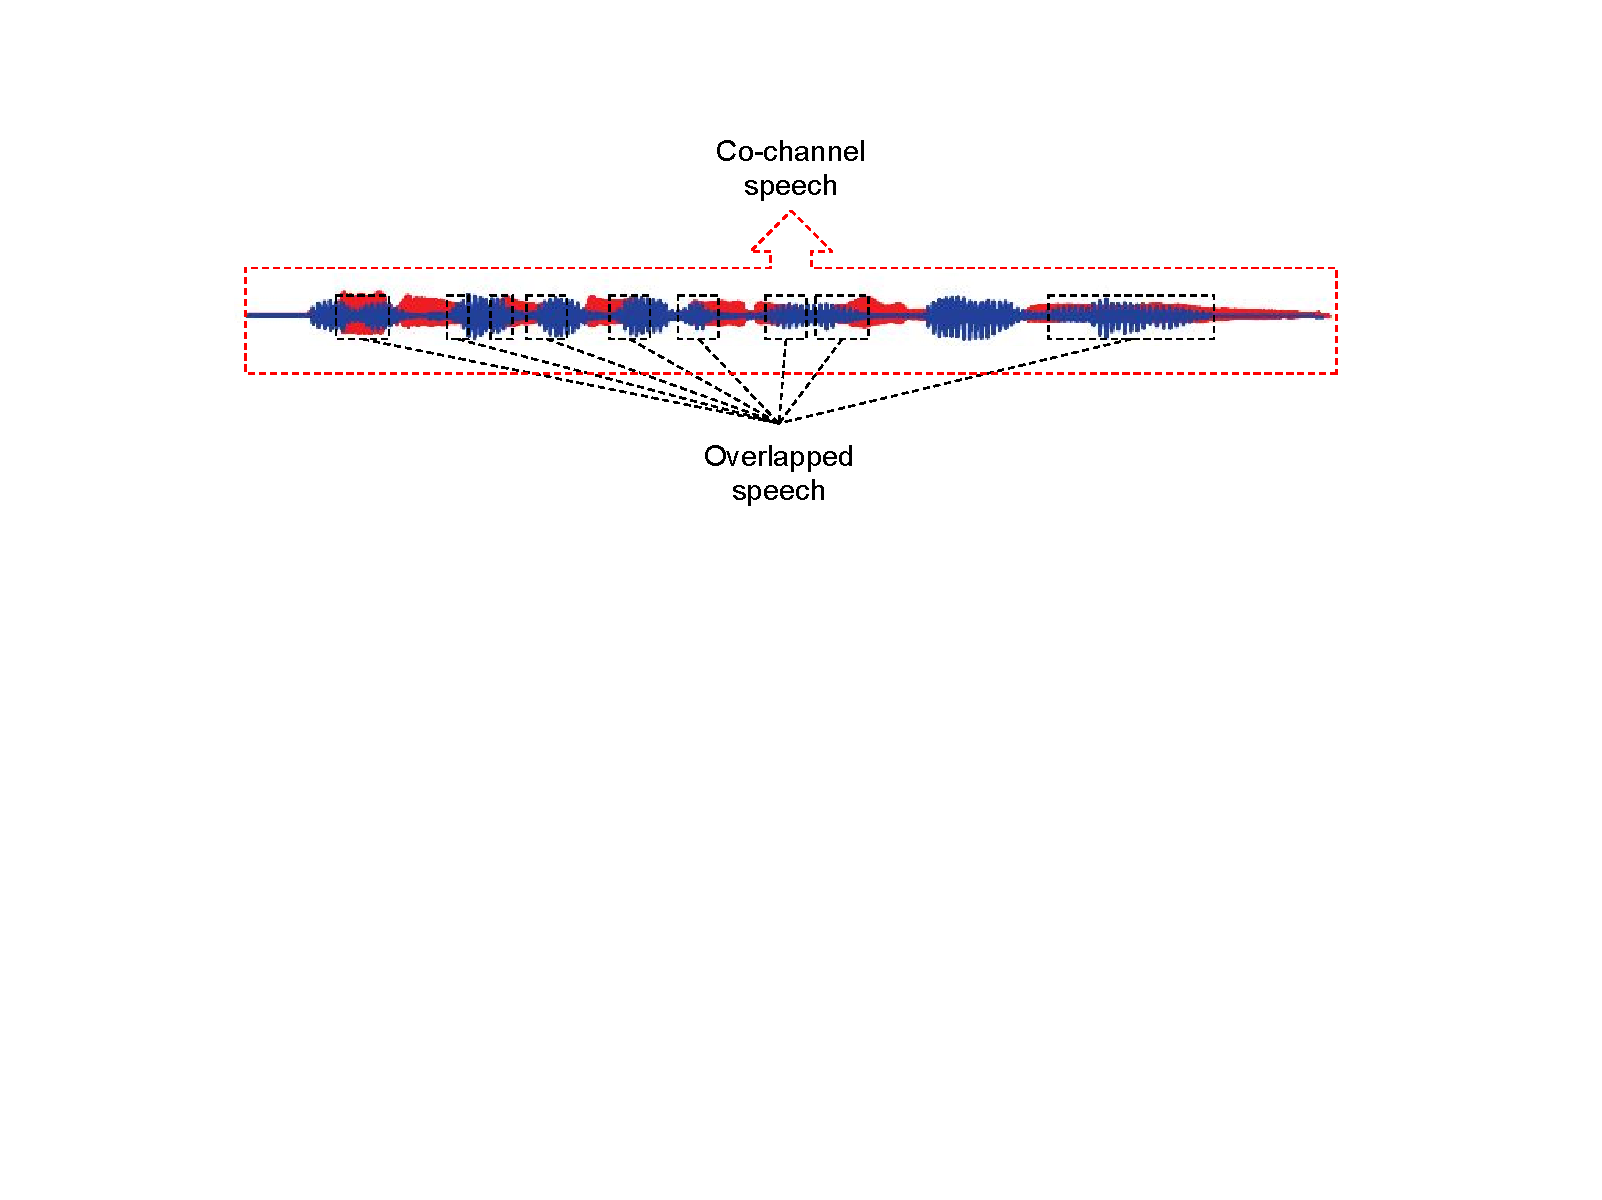
\includegraphics[height = 2in, width=0.9\textwidth]{figures/cochannel_vs_overlap-crop}
	\vspace{-3mm}
	\caption{\it \small Difference between co-channel and overlapped speech. Overlap refers to instances where more than one speaker is active. Co-channel is defined as an entire stream that contains multiple speakers. All co-channel files do not necessarily contain overlap. }
	\label{fig:cochannel_vs_overlap}
	\vspace{-3mm}
\end{figure}


%The specifics of recording conditions are overlooked in this study. 
%For example, information that relates to each speaker’s distance from the microphone and room acoustics. 
%This is intentional, since most of the difficulty in dealing with co-channel speech arises 
%from it being single-channel, which implies limited access to spatial 
%information as well as other sources of meta-data.

Aside from overlapped vs. non-overlapped speech, there are different ways of categorizing co-channel data in terms of how it is generated. 
Among such is a semantic classification that focuses on speakers' interactions with each other and divides co-channel data into two subgroups: 
\begin{itemize}
	\item conversational co-channel speech
	\item co-channel speech with independent parties
\end{itemize} 

Conversational co-channel speech refers to recordings in which speakers acknowledge other parties in the recording and engage in dialog. 
Alterations of speech production are an important artifact of conversational co-channel speech, which are the result of conscious and unconscious reactions of the foreground speaker and interferer(s). 
Examples of such alterations are raised pitch and energy level ~\cite{Shriberg01observationson,schegloff2000overlapping}. 
Raised Pitch and volume are especially common at or around overlaps. 
Readers are probably familiar with political debates with heated arguments. 
Most debates are perfect instances of an exaggerated version of the above-mentioned changes in speech production. 
Schegloff argues that long and sustained overlaps are primarily a sign of argumentative speech~\cite{schegloff2000overlapping}. 
In such conversations, most speakers tend to alter their voice in order to control the floor. 
These changes are problematic in automatic speech applications and are considered a type of distortion. 
Treatments are directed towards applications that suffer the most from speech alterations, predominantly automatic transcription of speech, i.e., speech recognition. 
Aside from changes in speech production, the element of interference by competing speakers is also an important artifact observed during overlaps. 
Therefore, in conversational co-channel data, one has to consider both overlaps and speaker specific alterations as sources of distortion and mismatch. 

Co-channel data with independent parties, are examples of co-channel data where the speakers do not interact with each other. 
An example of this types is cross-talk between separate channels; imagine switching between radio stations on an analog AM radio. 
The main characteristic of such data is that speakers are not aware of each other and therefore do not pertain to normal conversational mannerisms. 
That includes following turn-taking rules, which in most cases limits overlapped speech. 
Artificially generated co-channel data (mixing independent channels) is another example of co-channel speech with independent parties. 
A considerable portion of this study will focus on this type of co-channel data to analyze performance of overlap detection and also speaker recognition. 
We rely on this type of data since it provides the flexibility of controlling the amount of overlapped speech. 
As we will show in the next chapter, conversational co-channel speech does not necessarily contain sufficient overlapped data for some of our experiments. 
Therefore, we allow ourselves to neglect some aspects of conversational co-channel speech for the benefit of more overlap. 
That is why we value ``co-channel data with independent parties'', despite some of its unrealistic characteristics compared to conversational speech. 

The treatment of different speech processing applications for co-channel speech will focus on one of the two categories described above. 
This study will focus on a number of speech applications including: 
\begin{itemize}
	\item Signal processing and audio classification: identifying and separating overlapped segments in co-channel files. 
	\item Speaker recognition/verification: The ability to automatically decide whether two or more speech samples belong to the same speaker. 
	\item Speaker diarization: Segmenting an audio stream by counting the number of speakers as well as determining who spoke when. 
\end{itemize}

A description of an outreach to signal processing in vehicles is also presented, where algorithms developed for co-channel speech analysis were used to improve driver safety. 

\section{Approach}

The goal of this thesis is to provide tangible solutions to problems caused by co-channel speech in automatic speech technology. 
We argue that part of these issues are caused by overlapped speech (direct speech interference), which plays a significant role in making co-channel speech a difficult problem. 
The presence of overlapped speech can be detrimental to speaker diarization and speech recognition systems. 
%There is no clear and unique way of labeling or transcribing overlapped segments. 
In speaker diarization, it becomes difficult to assess system performance at overlaps, due to the inherent ambiguity in labeling overlapped segments. 
The same goes for speech recognition where aside from determining which is the ``primary'' speaker, recognizing speech at overlaps is more difficult, due to interference coming from other speakers. 
For this and other reasons detailed in the next chapter, the first portion of this study is devoted to overlapped speech detection. 
Our approach to overlap detection will be to focus on developing signal processing techniques to detect and separate overlap from single-speaker speech. Figure~\ref{fig:overlap_applications} depicts some applications of overlap detection in speech technology. 

\begin{figure}[h!]
	\centering
	\vspace{0mm}
	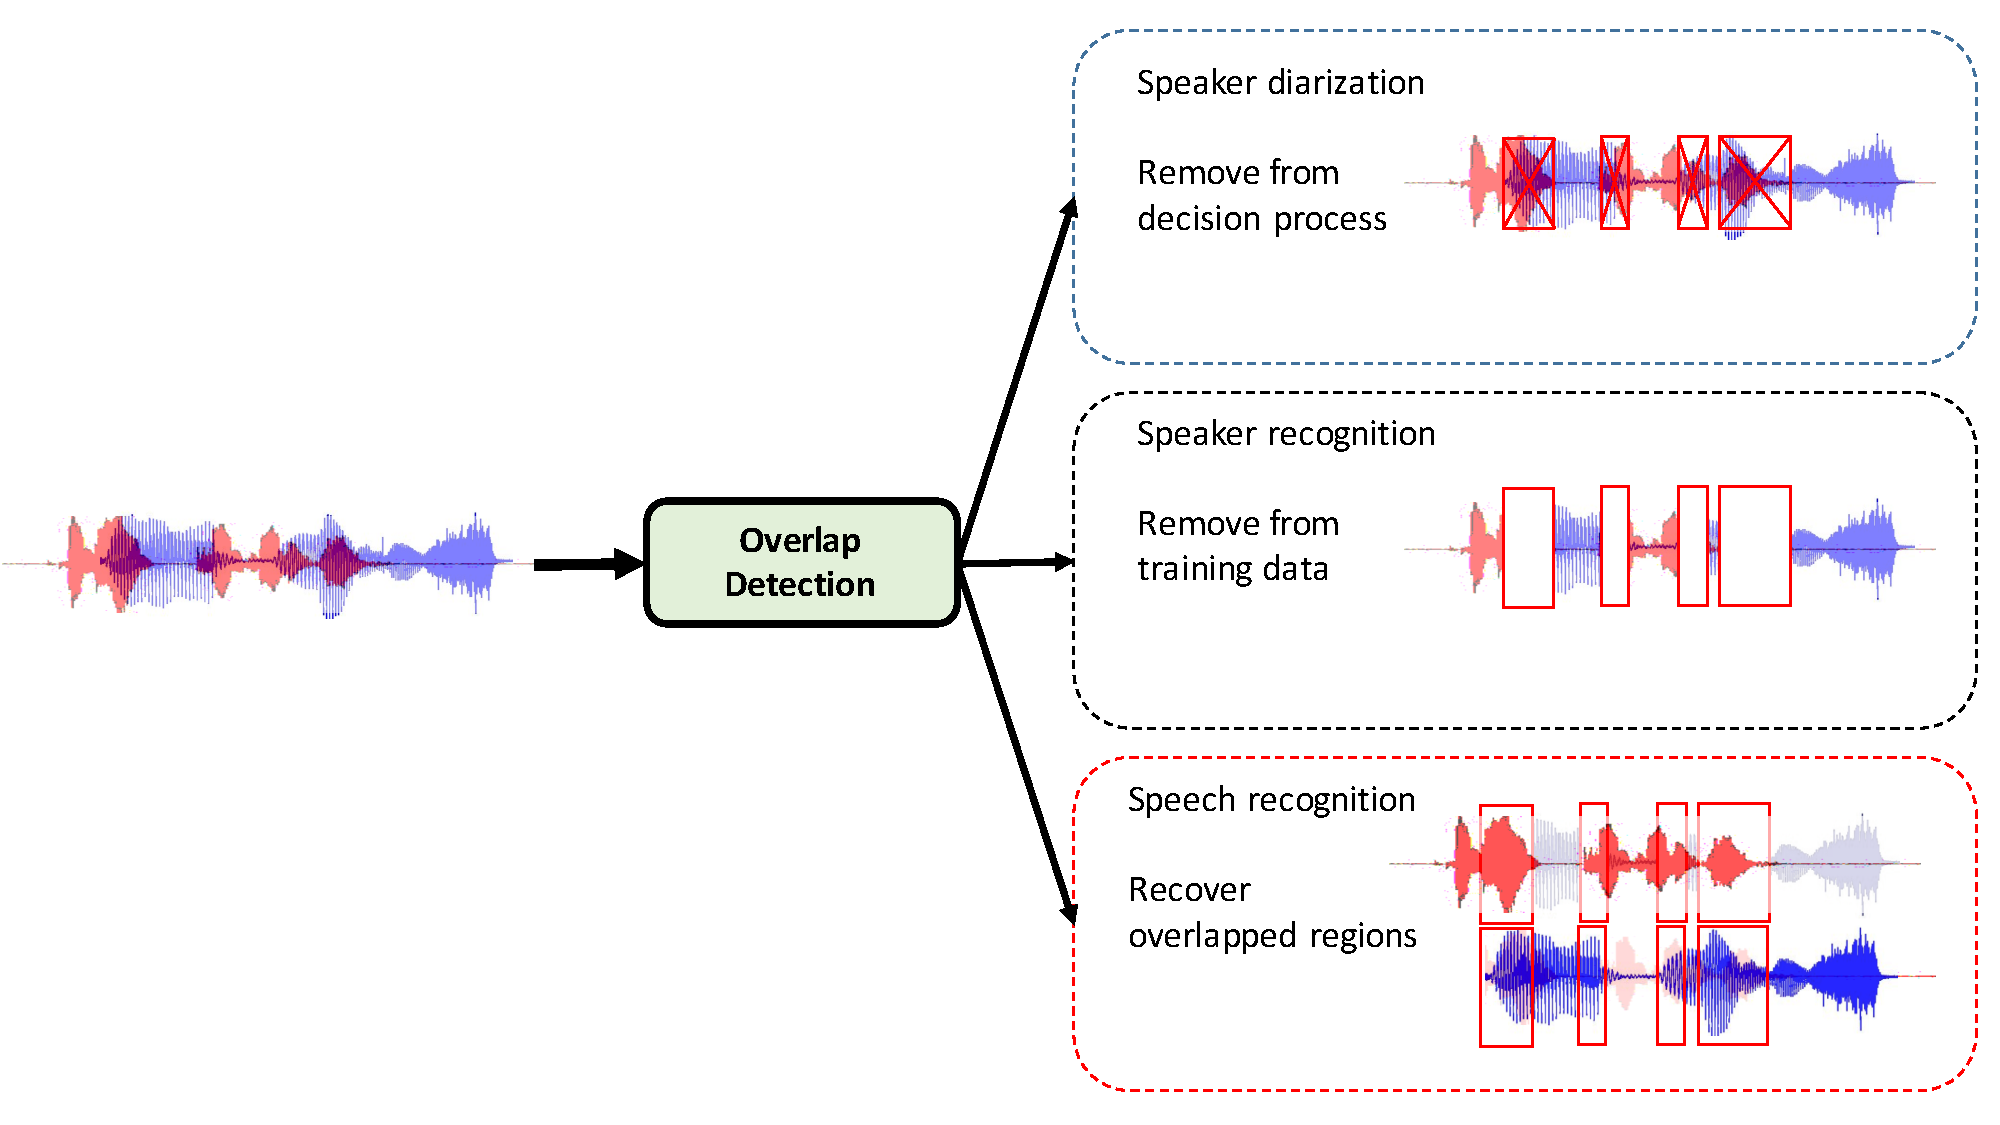
\includegraphics[height = 3in, width=\textwidth]{figures/overlap_detection_applications}
	\vspace{-3mm}
	\caption{\it \small Various applications of overlap detection. Top: In speaker diarization, ignoring overlapped regions provides a more fair assessment of diarization performance. Middle: Removing overlaps in speaker recognition increases the reliability of training data. Bottom: Overlap detection results can be used as an initial step to recover overlapped regions.}
	\label{fig:overlap_applications}
	\vspace{-3mm}
\end{figure}

Although overlap is considered an important aspect of co-channel speech, in many conversational speech data, the amount of overlap can be considered negligible, depending on the application. 
One such application is speaker recognition, which is also the main theme of this thesis. 
In text-independent speaker recognition, speech content (i.e., what is being said) is of less values compared to long-term speaker dependent characteristics (i.e., who is speaking). 
The standard approach in dealing with co-channel speech in such cases is speaker diarization. 
The role of diarization is to segment audio streams into shorter intervals each of which contains only one speaker. 
We consider speaker diarization a ``signal level'' approach. 
The term signal level is in respect to co-channel speech, since it is removed from the original signal prior to any other processing.
Alternately, a novel approach is presented in this study with the intention of bypassing the use of speaker diarization in the aforementioned scenario while preserving speaker recognition performance. 
This approach is to remove unwanted speaker-dependent information from latent variable subspaces generated from audio files~\cite{dehak2011front,kenny2010bayesian}. 
We refer to such solutions as ``subspace level''. 
Therefore, chapters III and IV each propose a different approach to remove interfering speakers from co-channel data. 
\begin{enumerate}
\item Remove interfering speakers in the feature subspace level: i-vector subspace factorization (Chapter III).
\item Remove interfering speakers in the signal level: speaker diarization (Chapter IV).
\end{enumerate}

Speaker diarization, will attempt to recognize and group speech that belongs to the same speaker in a co-channel audio stream. 
While subspace factorization maps speaker-dependent models to a subspace that will only contain parameters identifying the speaker of interest (aka primary speaker). 
Once again it should be pointed out that the main theme of this study is to address speaker recognition and identification in co-channel speech. 
Which makes speaker diarization an inseparable part of our approach. 


